\chapter{NFC Usage In Health Tech, Android NFC \& Privacy}
\label{chap:ch2}

\section{NFC Technology}
\label{sec:ch2sec1}

\par Near Field Communication (NFC) is a standards-based short-range wireless connectivity technology that makes life easier and more convenient for consumers around the world by making it simpler to make transactions, exchange digital content, and connect electronic devices with a touch. NFC is compatible with hundreds of millions of contactless cards and readers already deployed worldwide. \cite{whatIsNFC}

NFC is distinct from far field RF communication that is used in personal area and longer-range wireless networks. NFC relies on inductive coupling between transmitting and receiving devices. The communication occurs between two compatible devices within few centimeters with 13.56 MHz operating frequency. \cite{coskun2013survey}

We have to remember that there are three major devices in NFC: NFC enabled mobile phones, NFC readers and NFC tags. NFC communication occurs between two NFC devices with some valid combinations. For example a mobile phone may communicate with a NFC reader. \cite{coskun2011near}

As the communication method of NFC is a very close range one it is very common that the user will actually touch their phone to the NFC reading device or NFC tag. That's why this process might also be known as the touching paradigm. The user must always be aware in order to perform near field communication, as the user needs to actively "touch" the other communication device, being it either a NFC reader, a tag, or another NFC enabled phone. A NFC tag can be seen in figure \ref{fig:nfc-tag}.

\begin{figure}
\centering
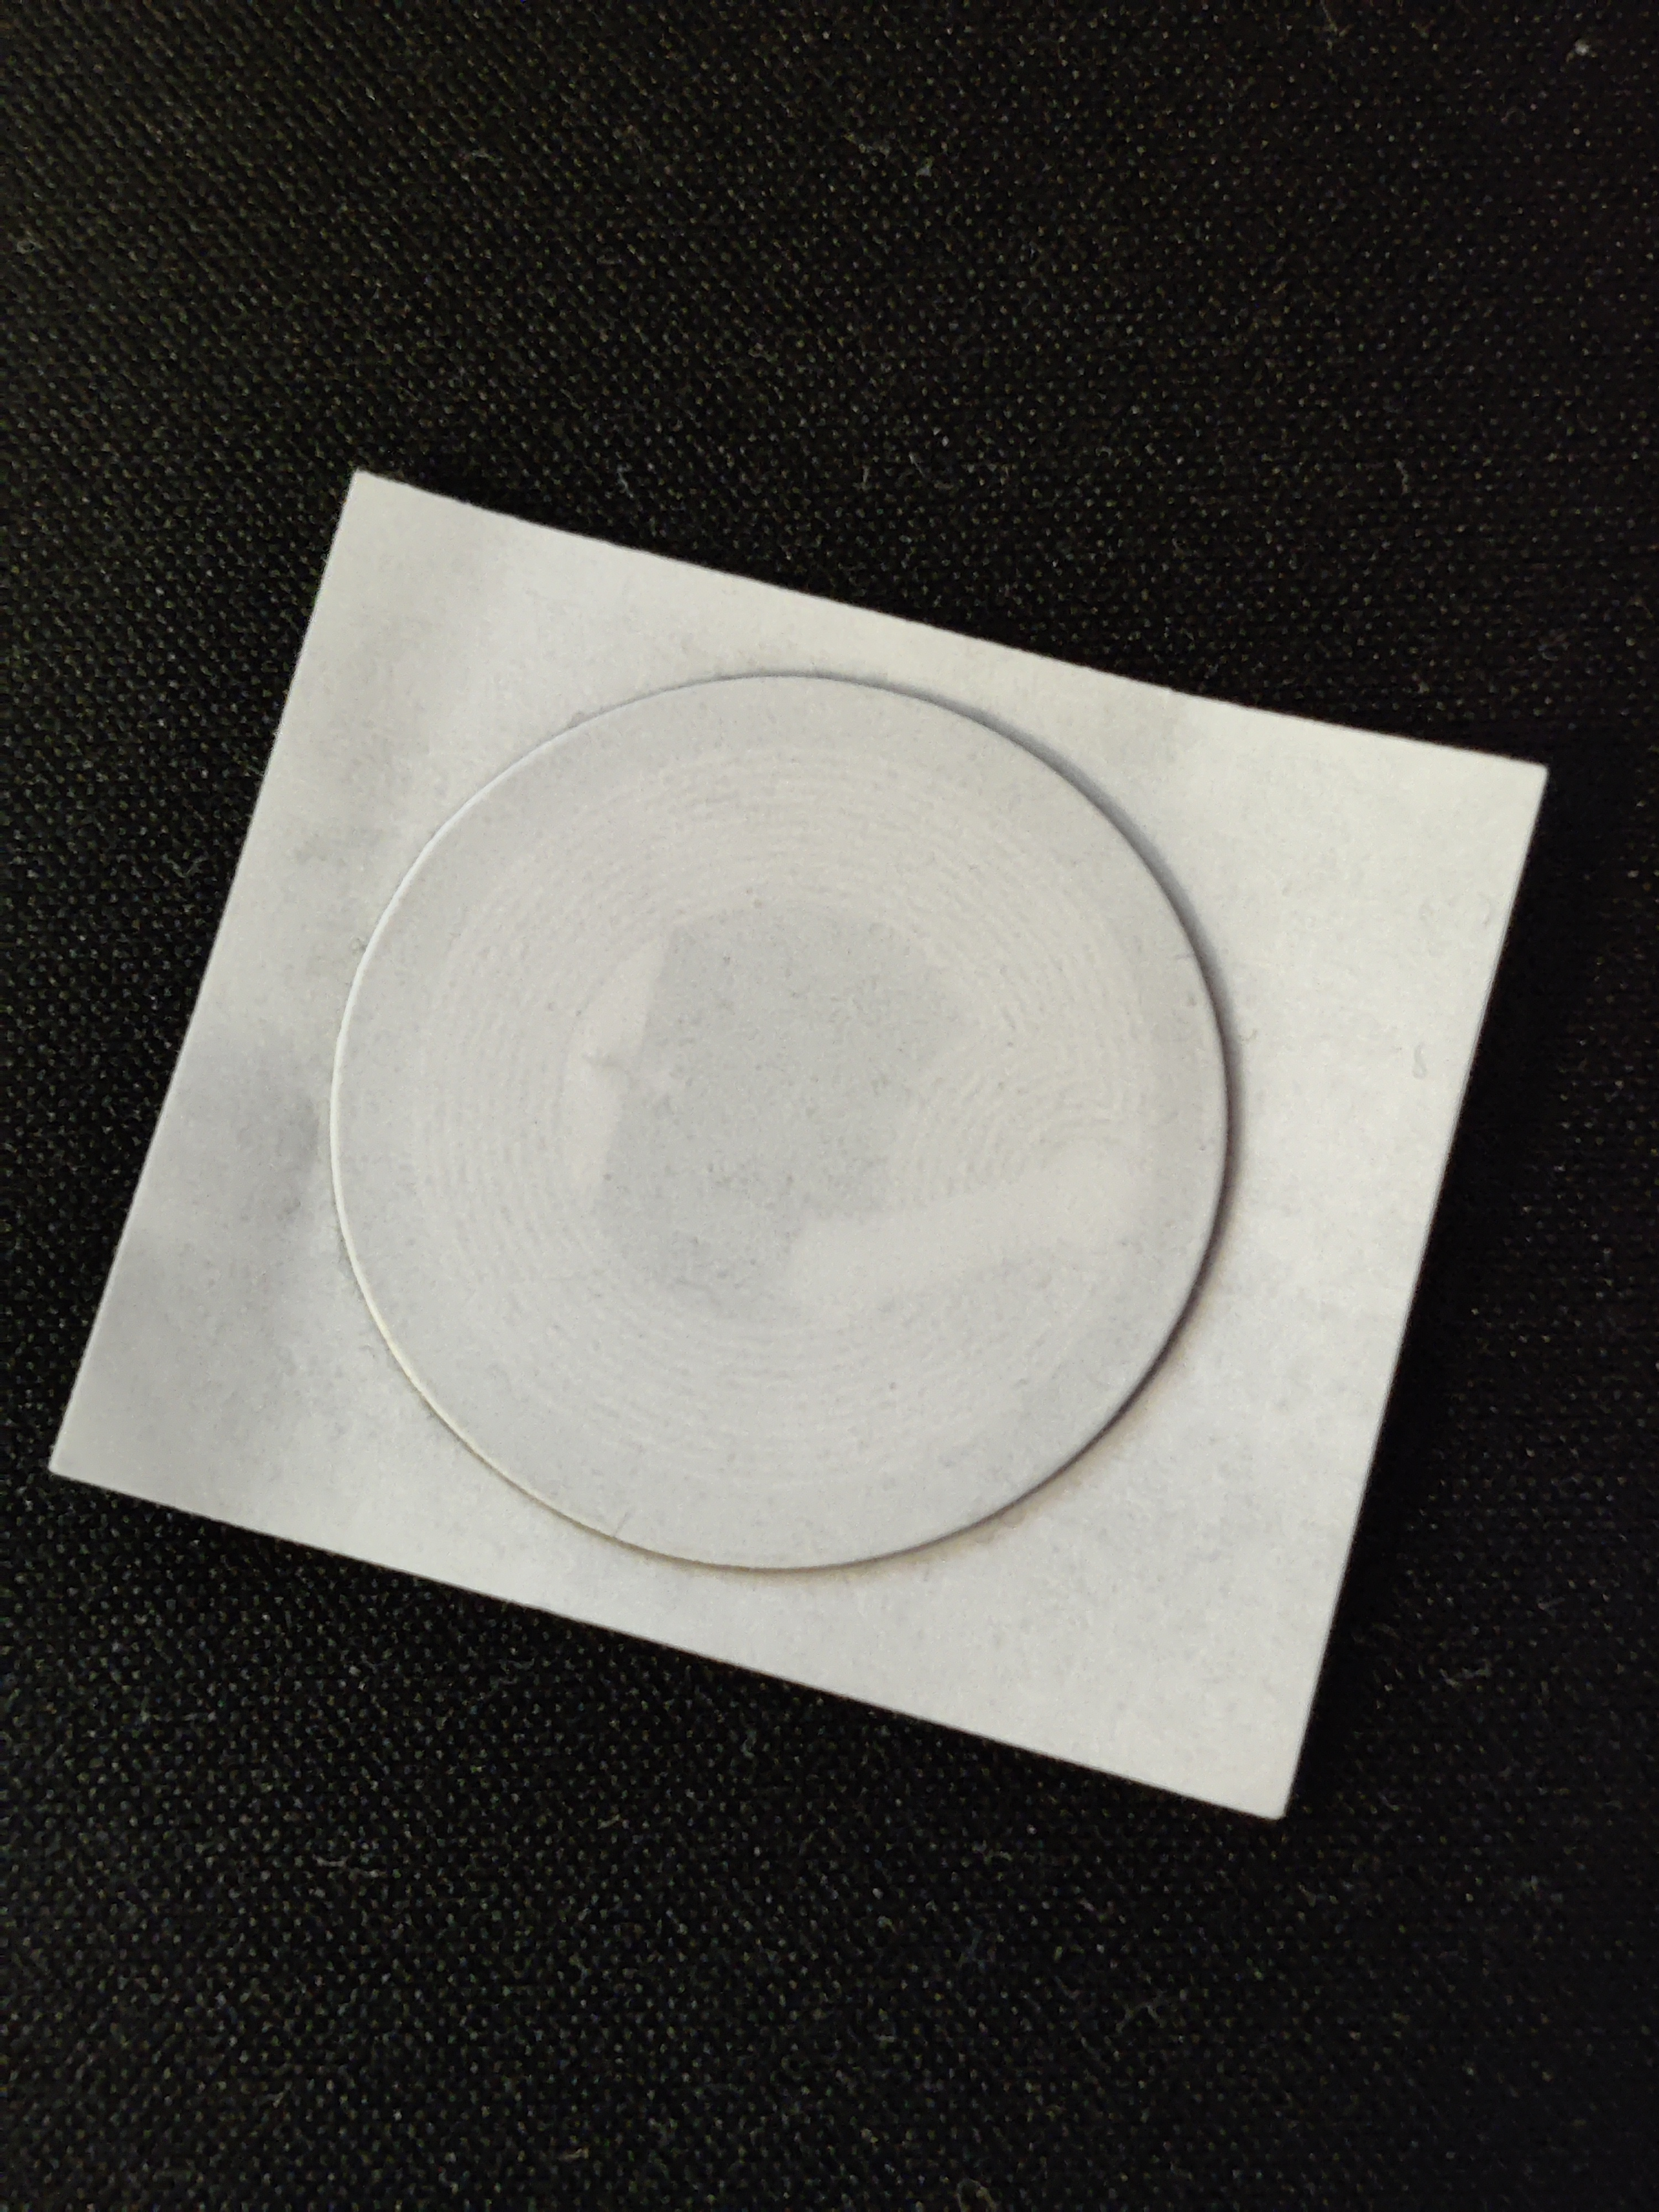
\includegraphics[width=0.4\textwidth]{figures/nfc_tag.jpg}
\caption{NFC Tag}
\label{fig:nfc-tag}
\end{figure}

As a result of a NFC event an exchange of data is being done, for example: in case of a phone communicating with a NFC enabled point of sale (POS, can be seen in figure \ref{fig:pos}) the phone will send the card information needed in order to complete that specific transaction and it will receive a confirmation from the POS. The contactless payments is merely one of the many amazing things that can be done using the NFC technology though.

\begin{figure}
\centering
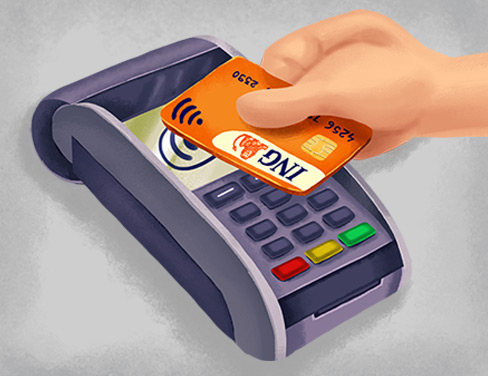
\includegraphics[width=0.4\textwidth]{figures/pos.jpg}
\caption{Point Of Sale (POS) \cite{posImage}}
\label{fig:pos}
\end{figure}

\section{NFC Android}
\label{sec:ch2sec2}

\par The first device to provide NFC functionality was the Nokia 6131 phone in 2006. However the Android operating system was only introduced in 2008 and it took 2 years for an android phone to be equipped with NFC support and the first android phone to do it was Samsung's NEXUS S, released in 2010.

As it is mentioned in \cite{nasution2012prototype}, the function of NFC was introduced by Google into Android 2.3 (API level 9) device. In Android 2.3, the ability of device is limited in only reading the tag. In Android 2.3.3 (API level 10), data writing and trading ability through mode Peer to Peer (P2P) began to be implemented within android devices. 

The uses of the NFC in the Android space are vast and useful in many different ways. One of those is of course the Google Pay system which allows you to make contactless payments with the cards saved into your Google accounts. There was another very interesting feature in Android, called Android Beam which allowed you to transfer files between two NFC enabled Android devices just by touching them one to the other. However, this was deprecated with the introduction of Android API level 29 (also known as Android Q or 10) and replaced with Google's new addition, Nearby Share, which is a direct response and competitor to Apple's AirDrop.

File transfers and contactless payments are merely the top of the iceberg though, the more interesting thing about it comes when you add into the equation the NFC tags. Those can easily be written to with free applications from the Google Play Store, such as TagWriter which allows you to store information or even different commands on the tags. You can use them to store contacts, web pages, or WiFi connectivity information in a manner that when you tap such a tag your device will automatically prompt you to connect to the specific network that has been stored on that specific tag without the need for you to introduce a password (as long as you are in the range to do so, of course).

Another very frequently used functionality of the NFC on Android devices is for pairing bluetooth devices with the mobile phone, such as NFC and bluetooth enabled speakers or even cars. The possibilities are limitless as you can implement custom functionalities.

When NFC was first introduced there were serious concerns about security and privacy, however Google gave the users full control on whether their device can read and receive information throughout the NFC functionality or not by simply adding a toggle button in the quick settings, similar to the WiFi toggle button, see figure \ref{fig:nfcToggle}.

\begin{figure}
\centering
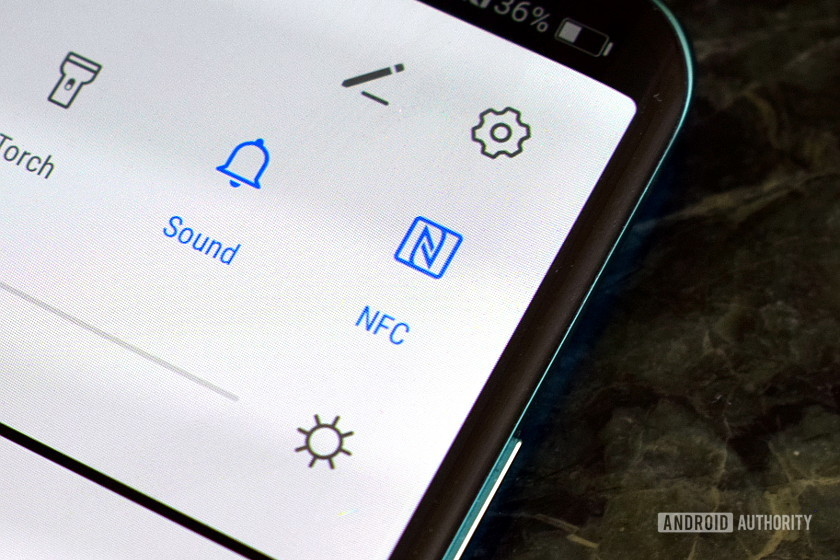
\includegraphics[width=80mm]{figures/nfc_toggle_button.jpg}
\caption{The NFC Toggle button on an Android device \cite{howToUseNfc}}
\label{fig:nfcToggle}
\end{figure}

\section{Usage of NFC in health and other domains}
\label{sec:ch2sec3}

\par As stated in the sections \ref{sec:ch2sec1} and \ref{sec:ch2sec2} one of the domains where the Near Field Communication technology thrives is payments. It was first introduced in the so called contactless cards, which is just a simplified name, easier to recognize by the public, for a Near Field Communication (NFC) enabled card. Those were a serious security concern and people would be skeptical about them as a result of the fact that to make a payment you wouldn't be required any extra information, like the PIN code you would be required to introduce in order to confirm a normal card payment. However this was not true, at least not entirely, as payments without introducing a PIN code in order to confirm the transaction were not allowed past a certain amount, chose by the card issuer.

The NFC technology is also being used in ticketing and loyalty services such as bus tickets that are stored on an NFC enabled card, or loyalty cards that provide you with points that can be spent in different shops. It is also used in special card keys in order to provide you access in some rooms, like in hotels.

According to \cite{lazaro2018survey}, the inductance (and the corresponding capacitance) chosen in the tag design has an important role in the energy harvesting and the loading effects between the tag and reader. This interest in passive NFC sensors led manufacturers of integrated circuits to present several ICs (integrated circuits) with energy harvesting, thus demonstrating the potential market for this technology.

In accordance with \cite{steffen2010near}, if we have a car key with a NFC Interface, where the NFC interface is located inside the car’s key (connected to the key electronics), then one exemplary use case is the Car Status. When a user turns off the car, the car transmits status information to the key via the internal radio interface. When the user is outside the car, he can use a NFC mobile phone to read this information from the key like the status of the locks, the position of the car, the tank level etc.

A new functionality that Apple and Google both announced in the last year is the ability to store your car key on your phone, in order for you to be able to use your phone to unlock and start the car. However, the cars are not NFC enabled by default, so you would need a car that supports this technology in order to take full advantage of it. This will be widely available starting with Android 12, according to Google (figure \ref{fig:google-car-key}).

\begin{figure}
\centering
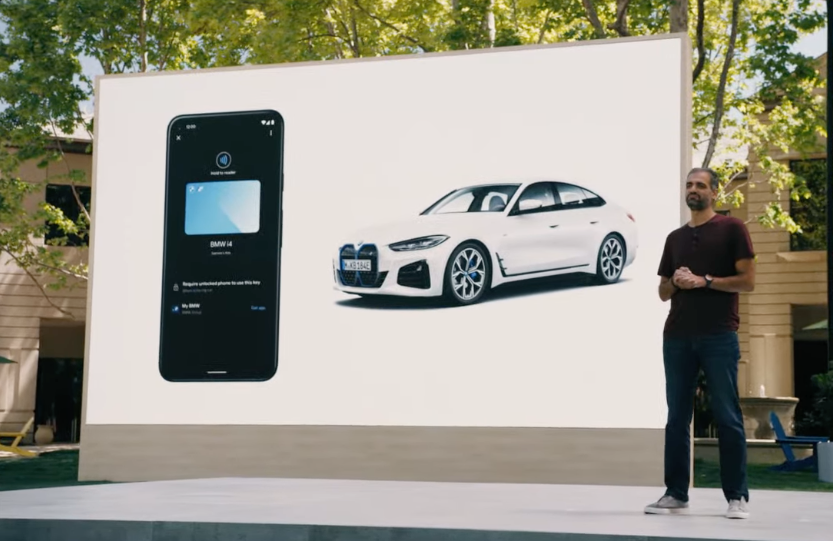
\includegraphics[width=\textwidth]{figures/google_car_key.png}
\caption{Google car key solution \cite{carKey}}
\label{fig:google-car-key}
\end{figure}

Consumers who own car models that have enabled NFC technology, or near-field communication, will be able unlock their car by tapping their phone against the door. The phone communicates with an NFC reader in the user’s car, which is typically located within the door handle. Google said users will also be able to securely and remotely share their car key with friends and family if they need to borrow the car. \cite{carKey}

When it comes to health care the NFC technology is not yet used, however there are studies that explore the ways RFID (Radio-Frequency Identification System) and NFC (which is an RFID based technology) could be used in order to make certain parts of the patient treatment easier and more error-free. One of those parts is actually the medication which is prone to errors due to it being quite demanding in the way it should be administrated. The safe medication care is based on five ”rights”: right medication, right patient, right dosage, right way of taking medication, and right time. \cite{lahtela2008rfid} Using the NFC technology three of these "rights" would be quite easy to accomplish, those being the right patient receiving the intended medication in the prescribed dosage.

Figure \ref{fig:nfc-medication-system} shows how RFID could be used in medication care combined with the electronic patient record and a data system. Tags are placed onto the patient and onto the medication, which information the nurse reads with RFID reader. Next the information is transmitted to the data system for handling, from which the data finally continues to the electronic patient record and to the nurse. The information, which is automatically read from the medication and from the patient to the electronic patient record, improves the surveillance of medication care. \cite{lahtela2008rfid}

\begin{figure}
\centering
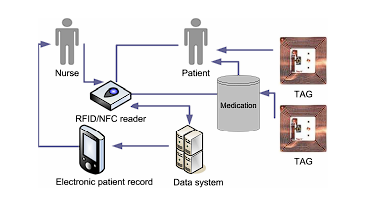
\includegraphics[width=0.75\textwidth]{figures/nfc_medication_system.png}
\caption{Using RFID/NFC in medication care combined with electronic patient record \cite{lahtela2008rfid}}
\label{fig:nfc-medication-system}
\end{figure}

The above scenario is just the start of what we can accomplish in the health care system using the NFC technology and stopping here would be a stupid thing to do. So what else can be done? Well the patient's tag could also contain other information than the prescribed medication alone and with a centralized server this could be just a reference to an entire database of information on one patient alone, including potential allergies, past interventions, blood related information and many other.

\section{Alternative to NFC usage in the Health Tech space}
\label{sec:ch2sec4}

\par As we stated in section \ref{sec:ch2sec3}, the Near Field Communication technology is not really used yet in the Health Tech space, not on a large scale anyway. This started us wondering, if not NFC, what are the alternatives used in this domain? As we were looking for any kind of answers we stumbled across iNTERFACEWARE and some other Electronic Medical Records (EMRs).

iNTERFACEWARE is a company that tries to help the hospitals and the public health agencies in storing their data securely while offering some integration solutions for their Iguana integration engine. Iguana is an amazing engine tool that was build specifically to meet the needs of today's medical system.

Alternatives to Iguana (by iNTERFACEWARE) are considered to be Adverity, EDI HQ and Workato. However none of the above are directly targeted towards the healthcare system. Adverity is targeted towards marketers in order to tackle their data challenges, EDI HQ is mainly designed to support clients in Retail, Logistics and, between others, Healthcare Industries. Workato is a workflow automation system designed for domains like HR, IT, Marketing and others. As a result of the mostly nonexistent alternatives we are either left with iNTERFACEWARE or some EMR solution provided by the Government (if there even exists such a thing).

While having the information stored on a remote server and accessible from certified laptops and desktops on a specific private network inside a medical center may be secure, getting those medical records and reports to the nurses or some other medical personnel is still a tedious job to accomplish using printed reports that are in some cases left at the bed of the patient or have to be requested every time from an information center in the hospital.

We can safely state that, even though EMR are a great solution for storing the information about patients in a secure way, the usage of printed reports that can sometimes be viewed or accessed by some random unauthorized person kind-of defeats the purpose of EMRs in the first place. We are not saying that those systems are not good, or not an appropriate solution, however we are saying that they are not enough by themselves and that those systems do not solve the entire problem on their own.

\section{Privacy concerns}
\label{sec:ch2sec5}

\subsection{Privacy in general}
\label{sec:ch2sec5subsec1}

\par First of all we need to answer a simple but rather complicated question: what is privacy? In order to answer this we turned over to \cite{solove2008understanding} for a better definition: "Privacy, however, is a concept in disarray. Nobody can articulate what it means. Currently, privacy is a sweeping concept, encompassing (among other things) freedom of thought, control over one’s body, solitude in one’s home, control over personal information, freedom from surveillance, protection of one’s reputation, and protection from searches and interrogations."

In a time where technology thrives and expands at a rapidly increasing rate, data becomes more and more important. As a consequence privacy is harder to preserve with each day passing by. Companies and institutes fight over how much information they can store about us for different reasons - some might be for a quality of service improvement, some for advertisements and other for the exact purpose of selling them and making a profit off of us. We believe that we can think of at least a handful of companies that do this. Let's take for example the three giants of the tech world: Google, Apple and Facebook. 

Facebook is by far the worst in the opinion of most people, especially since the Facebook-Cambridge Analytica data scandal from 2018. This specific event triggered a big concern around the world about consumer privacy and the data collected from the users which lead to an improvement in the legal system, especially in the EU, when the General Data Protection Regulation was enacted.

In 2018, the European Union, put into effect its new data protection law. The General Data Protection Regulation (GDPR) is the toughest privacy and security law in the world. Though it was drafted and passed by the European Union (EU), it imposes obligations onto organizations anywhere, so long as they target or collect data related to people in the EU. The regulation was put into effect on May 25, 2018. The GDPR will levy harsh fines against those who violate its privacy and security standards, with penalties reaching into the tens of millions of euros. \cite{whatIsGDPR}

Since this law was enacted there was a serious change in perspective around the world. People were more aware than ever about the importance of their privacy and they started demanding their rights. As stated in \cite{voigt2017eu}, the EU aims at regaining the people’s trust in the responsible treatment of their personal data in order to boost digital economy across the EU-internal market with the GDPR.

As a result of this fact the big giants, Google and Apple, took special steps in order to help preserving users privacy on the internet, but the one that surely affects us all is Google, as its advertisement system is the most used one on the internet. Recently they started working on a new data collection process in order to give users more privacy, while not completely giving up on targeted ads and their relevance to the user.

Google's proposed solution is called the Federated Learning of Cohorts (FLoC) which is supposed to take the place of the cookies we all know and love that you always have to allow in your browser whenever you access a website in order to have the intended experience. FLoC proposes a new way of targeting ads by no longer allowing the business to create a special profile on that person, instead it places a person in a cohort of users with the same interests. In this way you will still get advertisements for things that are relevant to you, but not as personal as before, for example:
if you've searched for let's say a Tesla Model 3 and a BMW i8, which are both electric cars, the algorithm will place you in a cohort of users that are interested in electric cars. As a result the ads targeted to your cohort will contain electric cars, but not necessarily the models you searched for or the brands you've searched for. Still relevant ads, but not as creepy as before.

\subsection{Privacy in the Health Care system}
\label{sec:ch2sec5subsec2}

\par Healthcare organizations store, maintain and transmit huge amounts of data to support the delivery of efficient and proper care. Nevertheless, securing these data has been a daunting requirement for decades. Complicating matters, the healthcare industry continues to be one of the most susceptible to publicly disclosed data breaches. In fact, attackers can use data mining methods and procedures to find out sensitive data and release it to public and thus data breach happens. While implementing security measures remains a complex process, the stakes are continually raised as the ways to defeat security controls become more sophisticated. \cite{abouelmehdi2017big}

We can see that we as a society started evolve in this specific subject of privacy in the last 3 years, yet there are still domains that need to catch up, in a big way. According to GDPR, hospitals have an even bigger than before responsability of keeping our data private from prying eyes and this is not an easy job. In a space where they need to have quick access to our information, the medication that was prescribed to us and other records that are essential for them in helping you get healthy once again, it might be close to impossible to preserve a patient's privacy. 

As noted in \cite{hathaliya2020exhaustive}, nowadays, security and privacy are the primary concern of the healthcare industry because of a tremendous amount of health data accessed and transmitted over the Internet. The internet is basically open to everyone in order to communicate and search for information, so as a result there is a possibility of various attacks on the data. In order to respond, the specialists started using cryptography as a counter-measure to those attacks.

Privacy of information collected during health care processes is necessary because of significant economic, psychologic and social harm that can come to individuals when personal health information is disclosed. \cite{barrows1996privacy} This is not an easy challenge and establishing such an implementation of security policies can be quite demanding in an Electronic Medical Record (EMR) system. However one of the goals we are trying to achieve with EMRs is to ensure the availability of health data for authorized persons and the prevention of unauthorized or unintended withholding of information or resources \cite{barrows1996privacy} which in our opinion is worth fighting for.

Until now, whenever someone was hospitalized they would keep some medical reports around your bed, which contain different information about the patient, like her/his current condition, some personal information and the treatment or medication they are supposed to receive. The medical reports were around their bed to make it easier for the nurse and the different doctors to communicate about how the patient's situation is evolving. Today that is not a solution anymore, privacy is important and, not respecting it, punishable in Europe. Also a file about a patient near their bed can easily be accessed by someone unauthorized or ill intended, which represents a security threat to the data collected by that specific health institute.

As we stated in section \ref{sec:ch2sec4} there are no complete solutions to this issue at this point. We took a look throughout a catalog of mobile applications that could even come close to a potential solution to this problem an we could only find some medical records applications for mobile devices, like the Multi-Profile Medical Records application found on the Google Play Store, but those were never built nor intended to be used by a medical institute. Those applications were intended to be used by the patient to take notes for themselves, so once again those do not present a solution for the exact purpose of our problem.

\subsection{Privacy concerns when using NFC in Health Tech}
\label{sec:ch2sec5subsec3}

\par One of the main concerns when using the NFC technology when it comes to privacy is the fact that the NFC tags can be read by any device with NFC reader capabilities. There is no way to make the information private in a way that only authorized devices could read those tags. While this is indeed true and it is a real problem it can be easily mitigated by encrypting the data stored on this tags or by not storing any sensitive data on them, in a way that only a person with authorized access to the server can access the private information.

Let us suppose though that an authorized device reaches the hands of an unauthorized person which can lead to leaks of information and that person having access to the database through the mobile application. In order to solve this issue a possible solution could be a Two Factor Authentication (2FA) system, where after a successful tag read an extra step would be required in order to access the information, for example the device's PIN code, pattern, fingerprint or face recognition, depending on the user's device settings.

Another privacy/security concern is what if one person from the medical personnel, so someone with authorized access, decides to leak some information by screen-recording or taking screenshots of patient's information or of some medical reports? Is there a way to mitigate such actions? The answer to those questions is yes, there is a solution. The Android operating system provides us with a flag (FLAG\_SECURE) that can be used in order to make those actions impossible. 

How does it work? The operating system will completely deny your possibility of taking screenshots on screens that have this flag attached, while in the case of screen recordings you would be able to actually perform this action, whenever you enter those flagged screens the screen recording will have a black overlay over the content from those screens so no information would be leaked. 

What about the preview that the system shows us when we open the recent applications screen? This, as well, is considered secured. As a consequence whenever you put the application in background and open the most recent applications, if the last opened screen was a secure flagged screen you would not be able to see any preview of the screen's contents, instead you would be presented with a white screen as a preview.

\section{Proposed solution}
\label{sec:ch2sec6}

\par We thought about what was the best approach to our issue, taking into account the fact that it has to be easy to implement and handy to use in order to make the integration as simple as possible and with the smallest cost possible while also being easy to use by any authorized medical personnel. We came up with a really interesting solution which takes advantage of the fact that most Android powered phones have NFC capabilities these days.

In our solution we did not focus on the server side of the issue, as there probably is already some EMR integration in a medical institute. Instead we focused on the mobile application to provide an idea of what could be possible with some basic Application Programming Interface (API) end-points that are pretty easy to implement on the server side.

The solution that we are proposing takes advantage of the already implemented bracelets in hospitals, by including an NFC Tag in those bracelets. Those tags will contain a database ID, with no meaning to any person that doesn't have access to the database or real life reference to that person.

The medical personnel would be allowed to see old reports and generate new ones for a specific patient, nurses would be able to register a new patient and write the id to the bracelet's tag. There is a lot of space for developing new use-cases and help the users have specialized options based on their assigned role in the application. We believe that this solution would help the medical professionals have an easier time being up to date with every single report that's being generated when visiting the patient, thus making their work a tad bit easier.